\documentclass[a4paper,11pt]{article}
\usepackage[margin=2cm]{geometry}

\usepackage[titletoc,toc,title,page]{appendix}
\usepackage[nodayofweek]{datetime}
\usepackage{cite}
\usepackage{graphicx}
\longdate

\usepackage{minted}
\usepackage{titlesec}
\usepackage{hyperref}
\usepackage{fancyhdr}
\pagestyle{fancyplain}
\fancyhf{}
\lhead{\fancyplain{}{M.Sc.\ Group Project Report}}
\rhead{\fancyplain{}{\today}}
\cfoot{\fancyplain{}{\thepage}}


\title{Implementation of attentional bistability of the dragonfly visual neurons in an intelligent biomimetic agent\\\Large{--- Final Report ---}}
\author{Juan Carlos Farah, Panagiotis Almpouras, Ioannis Kasidakis, Erik Grabljevec, Christos Kaplanis\\
       \{jcf214, pa512, ik311, eg1114, ck2714\}@doc.ic.ac.uk\\ \\
       \small{Supervisors: Professor Murray Shanahan, Zafeirios Fountas, Pedro Mediano}\\
       \small{Course: CO530/533, Imperial College London}
}

\begin{document}
\section{Centrifugal Small Target
Motion Detector Neuron 1 (CSTMD1)}
\subsection{Methodology}
The function of this module is to implement a multi-compartmental model of the actual CSTMD neuron that exists in dragonflies, with the hope that it will create an effect of selecting one target from many in the visual field. It takes input from the ESTMD and gives output to the pattern recognition module. The initial code was given to us by our supervisors, who had already shown that there is mutual inhibition of CSTMD1 neurons that could indicate target selection, but it was our job to connect it to the rest of the system and also, as a secondary goal, see if we could replicate the target selection effect observed in real dragonflies. The main issues in tackling this model were:
\begin{enumerate}
	\item Understanding he complicated nature of the morphologically-modelled CSTMD1
	\item Learning how to use the simulation environment of the CSTMD1 neurons (NEURON simulation environment)\cite{w13}
	\item Efficiently connecting this module with both the ESTMD and the pattern recognition module
	\item Generating key indicators to measure the performance and the plausibility of the module, in order to assist the user in assessing the function of this neuron
\end{enumerate}

Given that the CSTMD1 is multi-compartmental model with several parameters that directly or indirectly affect its activity and effect to a given input, we needed to first fully understand the given model before proceeding with any further decisions. Thus, we performed several tests in order be aware of all the plausible values that should be tried for each of the parameters.

Moreover, we had to consider what would be the best way to provide stimuli to the CSTMD1 neurons as an input from the ESTMD module. The NEURON simulation environment provides many classes as a connection to a model from an external input. After examining all the different possibilities we decided to use a leaky integrator (IntFire2() point process). We made this selection as it is an integrate and fire point process meaning that it allows the modification of the total current as a parameter which is what we required in order to connect the two modules. IntFire2() has also a quite straightforward structure compared to other similar but considerably more complex point processes. More specifically, the ESTMD module provides a time series of neuron spikes which is essentially an array of values each of which corresponds to a spiking rate per retina pixel. Thus, we initiated one leaky integrator for each pixel and provided the spiking rate as its total current. We then connected these point processes to each of the CSTMD neurons used for the simulation. In order to make our model as much biologically plausible as possible, we added some randomized delays to the connections of the leaky integrators with the CSTMD1 neurons with the aim of ensuring that the desired inhibitory effect will be achieved while neurons are provided with some stimuli. We also applied a spatial Gaussian distribution to the weights of these connections, increasing the relative weights of the pixels in the centre of the visual field compared to those on the edges, as this is the case with real dragonflies \cite{w13}.

With regards to the output, since the pattern recognition module requires a considerable number of spike trains as an input, we had to find a way to connect the 2 modules without severely affecting the speed and performance of the CSTMD1 module. Hence, given the morphologically large axon of the CSTMD1 neuron \cite{geurten} we decided that, instead of using as many neurons as the inputs required by the pattern recognition module, to apply a large number of electrodes to different compartments of the neurons and thus provide the adequate number of spike trains without limiting the biological plausibility of our model.

After successfully connecting the different modules, our next goal was to define key performance indicators for the CSTMD1 module in order to measure as accurately as possible its performance and also be able to modify the several parameters of the given model and observe their effect to the simulation. For this purpose, we created several plots which recorded the activity of different compartments of the neurons as well as their spiking rates. 

\newpage
\begin{figure}[H]
\centering
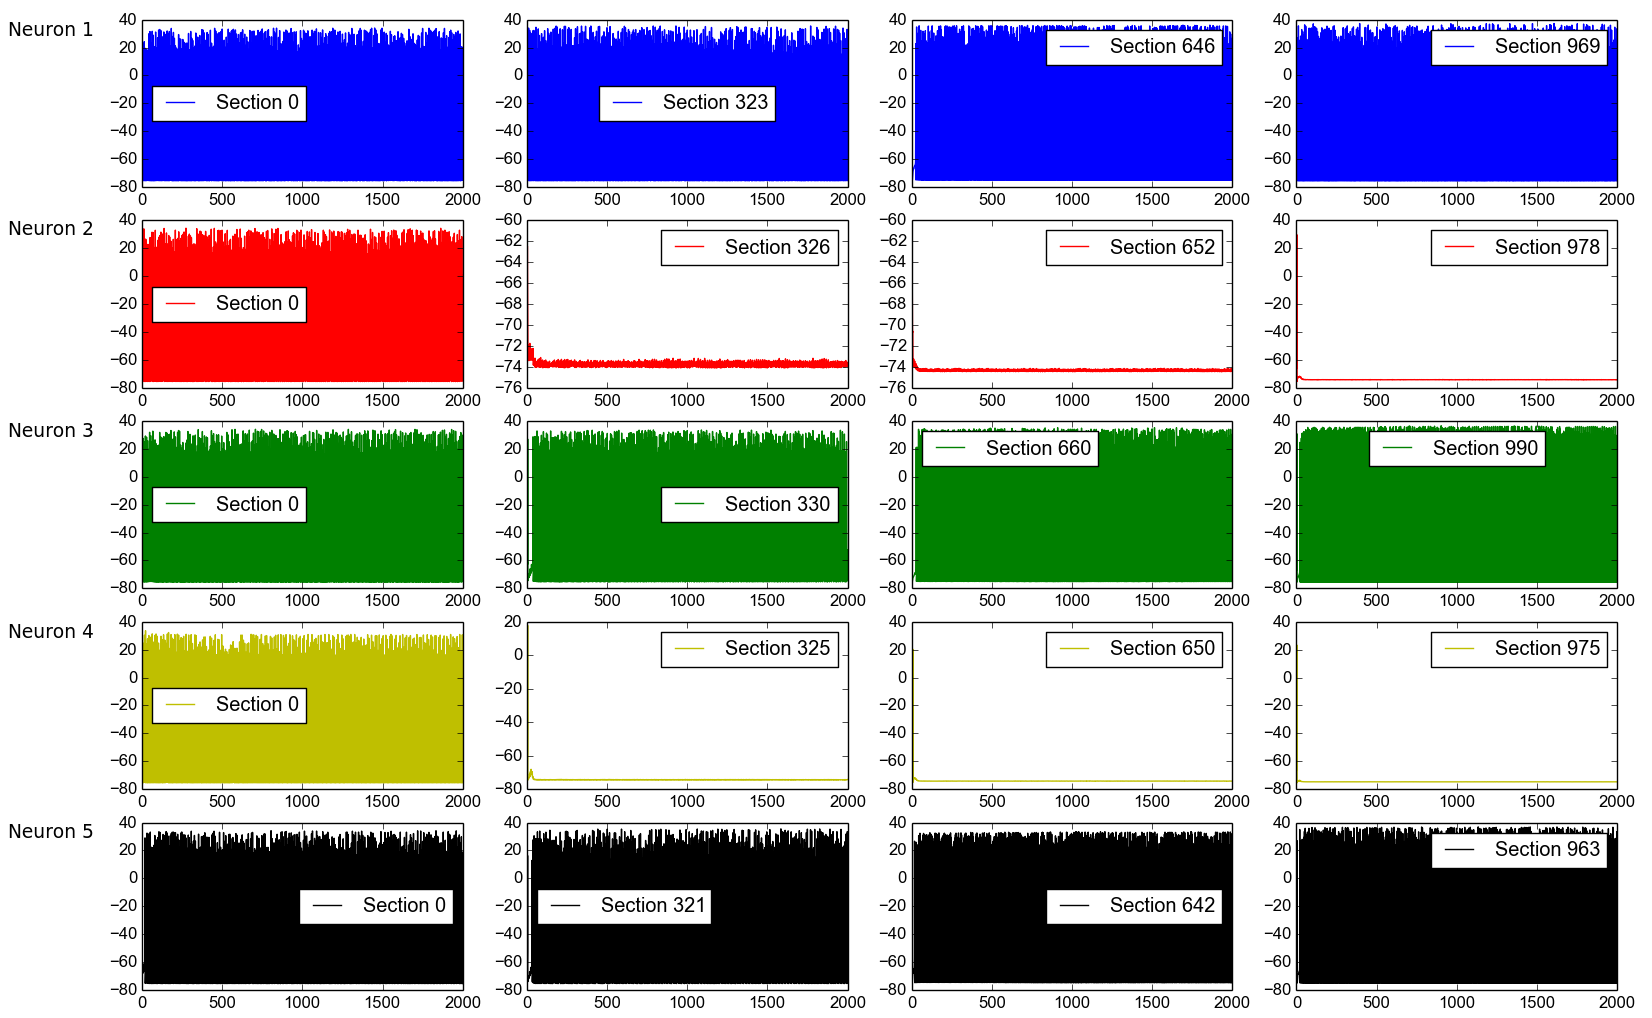
\includegraphics[scale = 0.3]{compartments}
\caption{Compartmental activity in a CSTMD1 neuron simulation showing inhibitory effects}
\end{figure}

The above figure shows the spiking rate of different compartments of 5 CSTMD1 neurons as these were used in one of our simulations in the NEURON simulation environment. We can observe that most compartments of the 2nd and the 4th neuron, coloured in red and yellow respectively, show little or no spiking activity although they seemed to have received similar stimuli to their counterpart neurons as it is shown by the spiking rates of their initial compartments in section 0. Hence, an inhibitory effect is evident which results in neurons 1,3 and 5 having high spike rates whereas neurons 2 and 4 show a blockade of activity.

We also extended the module to be able to run several simulations while given different inputs from the ESTMD module so as to observe if there is any evidence that our CSTMD1 module, when presented with two targets in the visual receptive field, would select one of them as we expected. However, after modifying all the possible parameters and trying different inputs, we observed that the CSTMD1 model is not displaying this selectivity.

\begin{figure}[H]
\centering
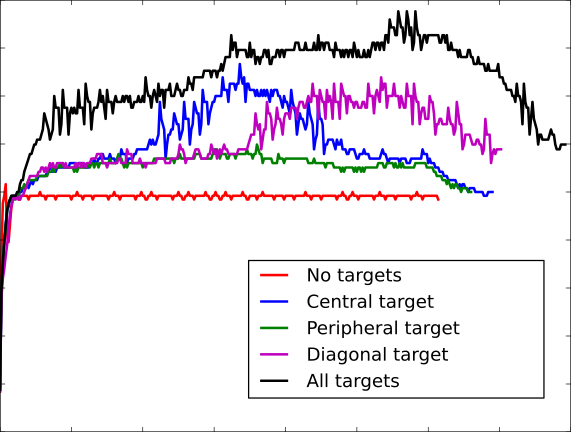
\includegraphics[scale = 0.5]{3targets}
\caption{Firing rates of CSTMD1 neurons given varius inputs}
\end{figure}

As it is shown in the above figure, we performed 5 different simulations in order to come to this result. We tried running the CSTMD1 simulation while giving different stimuli and we recorded their spiking rates. The lowest spiking activity is the one which corresponds to the simulation where no targets were presented. The blue, purple and green lines show variable spiking rates and correspond to simulations were targets in different positions were presented(central target, diagonal target and peripheral target respectively). However, when we performed a simulation were all targets were presented, the CSTMD1 neurons did not show any selectivity by resembling the spiking activity to the ones in the previous simulations and thus we were not able to replicate the results of \cite{w13}.Instead, what we are observing is a CSTMD1
neuron that fires more frequently when all targets are present.

The web client that we introduced supports running simulations of the CSTMD1 module. We transferred all the functionality as described above and thus the user is able to change all the significant parameters of the model and observe the resulting CSTMD1 neurons' behaviour as well as the behaviour of KPIs in the model.

\end{document}